\hypertarget{_trace_to_min_rdot_b_8c}{
\section{/home/mgh/LanlGeoMag/libLanlGeoMag/TraceToMinRdotB.c File Reference}
\label{_trace_to_min_rdot_b_8c}\index{/home/mgh/LanlGeoMag/libLanlGeoMag/TraceToMinRdotB.c@{/home/mgh/LanlGeoMag/libLanlGeoMag/TraceToMinRdotB.c}}
}
{\tt \#include $<$stdio.h$>$}\par
{\tt \#include $<$stdlib.h$>$}\par
{\tt \#include \char`\"{}Lgm/Lgm\_\-MagModelInfo.h\char`\"{}}\par


Include dependency graph for TraceToMinRdotB.c:\nopagebreak
\begin{figure}[H]
\begin{center}
\leavevmode
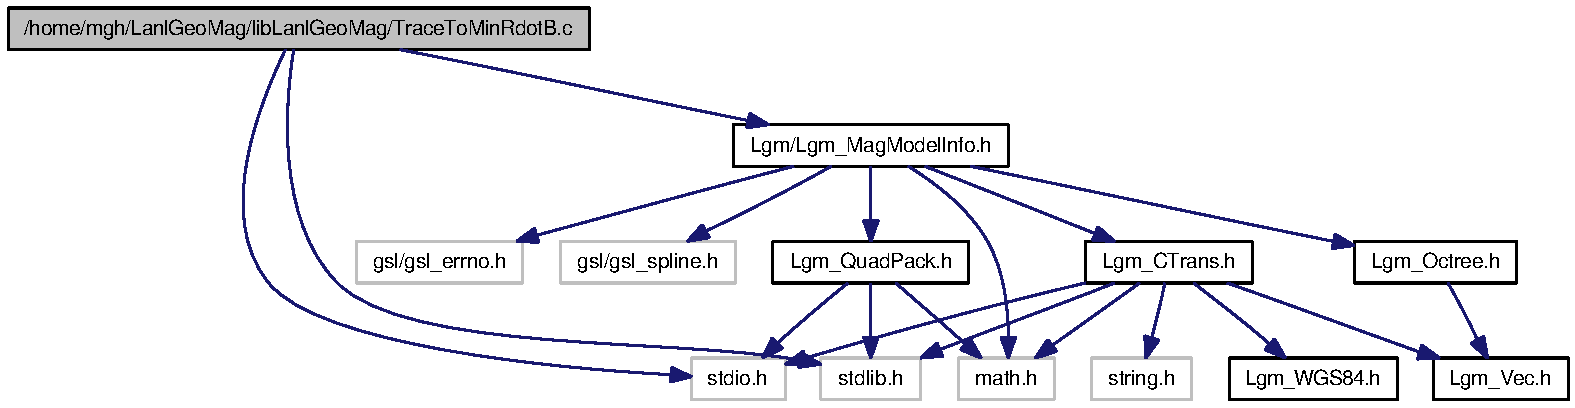
\includegraphics[width=396pt]{_trace_to_min_rdot_b_8c__incl}
\end{center}
\end{figure}
\subsection*{Functions}
\begin{CompactItemize}
\item 
int \hyperlink{_trace_to_min_rdot_b_8c_9c5db0561592bc1e8943696fbbd6dba2}{Lgm\_\-TraceToMinRdotB} (\hyperlink{struct_lgm___vector}{Lgm\_\-Vector} $\ast$u, \hyperlink{struct_lgm___vector}{Lgm\_\-Vector} $\ast$v, double tol, \hyperlink{struct_lgm___mag_model_info}{Lgm\_\-MagModelInfo} $\ast$Info)
\end{CompactItemize}


\subsection{Function Documentation}
\hypertarget{_trace_to_min_rdot_b_8c_9c5db0561592bc1e8943696fbbd6dba2}{
\index{TraceToMinRdotB.c@{TraceToMinRdotB.c}!Lgm\_\-TraceToMinRdotB@{Lgm\_\-TraceToMinRdotB}}
\index{Lgm\_\-TraceToMinRdotB@{Lgm\_\-TraceToMinRdotB}!TraceToMinRdotB.c@{TraceToMinRdotB.c}}
\subsubsection[{Lgm\_\-TraceToMinRdotB}]{\setlength{\rightskip}{0pt plus 5cm}int Lgm\_\-TraceToMinRdotB ({\bf Lgm\_\-Vector} $\ast$ {\em u}, \/  {\bf Lgm\_\-Vector} $\ast$ {\em v}, \/  double {\em tol}, \/  {\bf Lgm\_\-MagModelInfo} $\ast$ {\em Info})}}
\label{_trace_to_min_rdot_b_8c_9c5db0561592bc1e8943696fbbd6dba2}




Definition at line 21 of file TraceToMinRdotB.c.

Here is the call graph for this function:\nopagebreak
\begin{figure}[H]
\begin{center}
\leavevmode
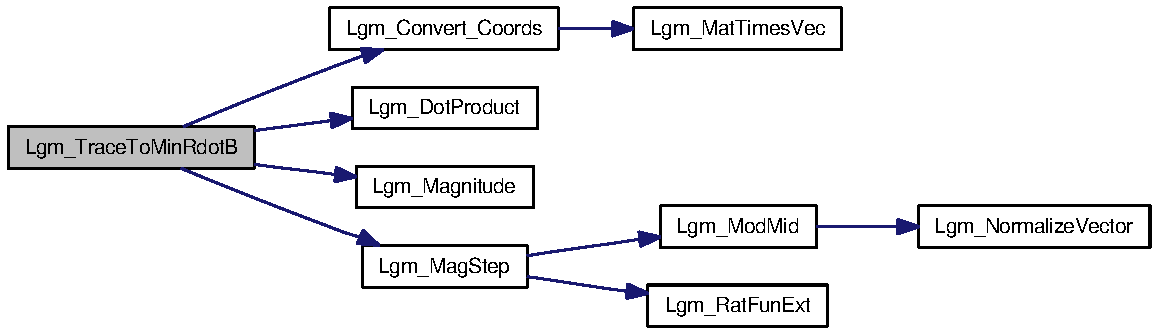
\includegraphics[width=296pt]{_trace_to_min_rdot_b_8c_9c5db0561592bc1e8943696fbbd6dba2_cgraph}
\end{center}
\end{figure}
